\documentclass[physics_notes.tex]{subfiles}
\begin{document}
\section{Aula 8 - 19/04/2023}
\subsection{Motivações}
\begin{itemize}
	\item Começar os estudos de dinâmica
\end{itemize}

\subsection{Exemplo de MCU - 67 Tiples}
Suponha que a Terra tem velocidade angular $\omega$ constante, velocidade e aceleração angulares $\vec{v}_{\theta}(t), \vec{a}_{\theta}(t)$
e velocidade e aceração escalares $\vec{v}_{e}(t), \vec{a}_{e}(t)$.
\begin{center}
	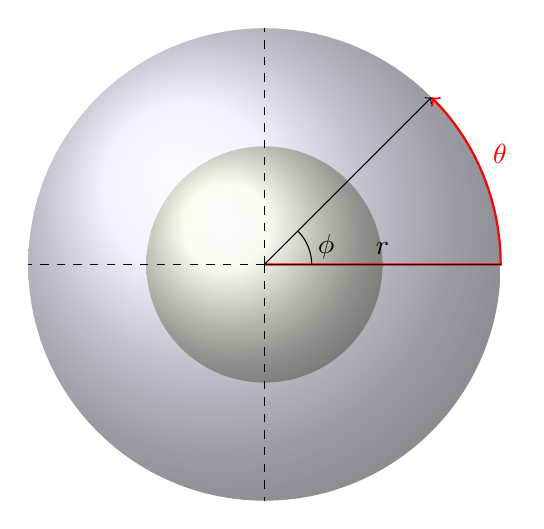
\begin{tikzpicture}[scale=3]
		\shade[ball color=blue!10!white,opacity=0.7] (0,0) circle (1cm);
		\shade[ball color=yellow!10!white,opacity=0.7] (0,0) circle (0.5cm);
		\draw[->,thick,red] (0,0) -- (1,0) arc (0:45:1) node[midway,above right]{$\theta$};
		\draw[dashed] (0,0) -- (-1,0);
		\draw[dashed] (0,0) -- (0,-1);
		\draw[dashed] (0,0) -- (0,1);
		\draw[->, black](0,0) -- ({cos(45)}, {sin(45)}) ;
		\draw (0,0) -- (1,0) node[midway,above]{$r$};
		\draw (0.2,0) arc (0:45:0.2) node[midway,right]{$\phi$};
	\end{tikzpicture}
\end{center}

No equador, $R_{E}=R_{T}, \omega_{E}=\omega$, tal que
$$
	\left\{\begin{array}{ll}
		v_{E}=\omega_{E}R_{E} = \omega R_{T} \\
		a_{E_{cp}} = \frac{v_{E}^{2}}{R_{E}} = \frac{(\omega R_{T})^{2}}{R_{T}} = \omega^{2}R_{T}.
	\end{array}\right.
$$
Na latitude $\theta,$ $R_{\theta} = R_{T}\cos{\theta}, \omega_{\theta} = \omega$, de modo que
$$
	\left\{\begin{array}{ll}
		v_{\theta} = \omega R_{T}\cos{\theta} \\
		a_{\theta_{cp}} = \omega^{2}R_{T}\cos{\theta}
	\end{array}\right.
$$
Para a Terra dar uma volta em torno de si de novo, ela demora aproximadamente 24h. Assim, $T = 24h$ é o período da Terra,
donde concluímos que a frequência será $f = \frac{1}{T} = \frac{1}{86400}s^{-1}.$ Como $\omega = 2\pi f,$ segue que
$$
	\omega = \frac{2\pi}{86400} = 7.27 \cdot 10^{-5}rad/s.
$$
Pede-se: a) Quais são os valores de $v_{e}, a_{e}?$ b e d) Quais são as orientações das acelerações? c) Quanto valem $v_{\theta}, a_{\theta}?$

a.) Vemos que $v_{E} = 463.1m/s, a_{E} = 0.0337m/s^{2}, g = 9.8m/s^{2}$. Em particular, $a_{E} = 0.0034g.$

b. e d.) O diagrama de v indica que o vetor aceleração aponta na vertical pra esquerda e levemente pra cima.

c.) Temos $v_{\theta} = 379.4m/s, a_{\theta}=0.0276m/s^{2}.$

\subsection{Dinâmica e Leis de Newton}
\subsubsection{O que esperar}
Quando estudamos os movimentos anteriores, estávamos vendo cinemática, a descrição matemática do movimento. No entanto,
nunca nos questionamos o que causa o movimento. Como ele surge, o que influencia-o, etc. Essa pergunta é respondida pela dinâmica,
q formulação matemática que explicíta as causas do movimento. Ela nos fornece uma relação entre as interações, chamadas forças,
que o corpo sofre e o seu movimento. A primeira formulação da dinâmica foi feita por Isaac Newton, sendo suas Leis nosso Ponto de partida.

\subsubsection{Leis de Newton}
A primeira Lei de Newton, também chamada de Lei da Inércia, afirma que
\begin{quote}
	``Um corpo em repouso, ou em movimento retilíneo uniforme, permenecerá em seu estado de movimento a não ser que uma
	força externa atue sobre ele. ''
\end{quote}
Observe que velocidade constante significa que tanto seu módulo será constante quanto a direção o movimento precisa ser em linha reta.
Uma consequência dessa Lei é que não tem distinção entre um corpo em repouso e um corpo se movendo com velocidade constante.
Com isso, um sistema de referencial inercial será definido como um eixo de coordenadas que está em repouso ou se movendo com
velocidade constante.

A segunda Lei de Newton surge para explicar como aparecem as forças dentro do contexto da dinâmica, dizendo que
\begin{quote}
	``A força resultante atuando em um corpo é igual à massa dele multiplicada pela aceleração''
\end{quote}
Matematicamente, isto significa que
$$
	\boxed{\vec{F}_{r} = m \cdot \vec{a} = m \cdot \frac{d \vec{v}}{dt}}
$$
O termo novo m é chamado de massa inercial, sendo interpretada como a grandeza física que expressa a resistência do corpo
ao movimento. Quanto maior for a massa, maior vai ser a resistência a se mover. De fato, se temos dois blocos de massas $m_{1}>m_{2},$ então
$$
	\vec{a}_{1} = \frac{\vec{F}}{m_{1}},\quad \vec{a}_{2} = \frac{\vec{F}}{m_{2}} \Rightarrow a_{1} < a_{2}.
$$
A dimensão dessa grandeza é $[m] = M$. No Sistema Internacional, a unidade de massa é o kilograma.

Note que a força é uma grandeza vetorial que soma-se, ou seja, se há várias forças agindo sobre um corpo, a resultante será
a soma delas. Se temos forças $\vec{F}_{21}, \vec{F}_{31}$ agindo sobre um corpo, então a resultante será $\vec{F}_{R} = \vec{F}_{21} + \vec{F}_{31}.$
Além disso, suas coordenadas serão
\begin{align*}
	 & x: F_{res}^{x} = -F_{21}\sin{\alpha} + F_{31}\sin{\beta}  \\
	 & y: F_{res}^{y} = -F_{21}\cos{\alpha} - F_{31}\cos{\beta}.
\end{align*}

\begin{center}
	\begin{tikzpicture}[scale=2]
		\draw[->,>=stealth, dashed] (-1.5,0) -- (1.5,0) node[right]{$x$}; % Draw the x-axis
		\draw[->,>=stealth, dashed] (0,-1.5) -- (0,1.5) node[above]{$y$}; % Draw the y-axis

		\draw (-0.75,-0.75) -- (0.75,-0.75) -- (0.75,0.75) -- (-0.75,0.75) -- cycle; % Draw the cube
		\draw[->,>=stealth] (0,0) -- (-1,-1) node[midway, below left]{$F_{21}$}; % Draw the F21 arrow
		\draw[->,>=stealth] (0,0) -- (0,-1) node[midway, right]{$mg$}; % Draw the gravity arrow
		\draw[->,>=stealth] (0,0) -- (1,-1) node[midway, below right]{$F_{31}$}; % Draw the F31 arrow

		\draw (0,-0.2) arc (-90:-45:0.2) node[midway, below]{$\beta$}; % Draw the angle beta

		\draw[dashed] (0,-0.75) -- (0,-1.5); % Draw the vertical dashed line for reference
	\end{tikzpicture}
\end{center}
A unidade da força é dada por $[F] = [ma] = MLT^{-2}$. No SI, sua unidade é $1kgms^{-2} = 1N$ o Newton.
Um corpo será dito em equilíbrio quando a força resultante agindo sobre ele é nula, pois, neste caso,
$$
	\vec{F}_{res} = \sum\limits_{n}^{}\vec{F}_{n} = 0 \Rightarrow F_{res} = ma = 0 \Rightarrow a = 0.
$$

A terceira e última Lei de Newton é conhecida como Lei da Ação e Reação. Segue seu enunciado
\begin{quote}
	``Se um corpo faz uma força em outro, então este segundo também realizará uma força no primeiro, sendo esta de
	mesmo módulo, mas com direção oposta. ''
\end{quote}
Em outras palavras, se um corpo 2 age sobre um corpo 1 com força $\vec{F}_{21},$ então o corpo 1 fará uma força sobre
o corpo 2 $\vec{F}_{12}$ tal que $\vec{F}_{21} = -\vec{F}_{12}, |\vec{F}_{21}| = |\vec{F}_{12}|$.

\subsubsection{Exemplo 4.2 - Tipler}
Os dados que temos é que há uma pessoa que se moveu 2.25m em 3s e cuja massa é 68kg. Pede-se para encontrar o módulo da força
agindo sobre ela. Segue que
$$
	x(t) = x_{0} + v_{0}t + \frac{1}{2}at^{2} \Rightarrow \Delta x = x(3) - x(0) = \frac{1}{2}a3^{2} = \frac{9}{2}a = 2.25m
$$
Isolando a equação, encontra-se que $a = 0.5m/s^{2}.$ Com isso, como $|\vec{F}| = |m \vec{a}| = 68 \cdot 0.5 = 34N$. \qedsymbol
\end{document}
